\chapter{Physcis Objects}

\label{ch:objects}
This chapter introduced the physics objects used in this thesis in the reconstruction of events. 
Boosted Higgs reconstruction is described in depth as several new techniques have been developed.
 The reconstruction of primary vertices is described in Section~\ref{sec:pv}. 
Different types of jets that are used by this analysis in different kinematic regions are described in Section~\ref{sec:jets}. 
The reconstruction of electrons and muons are described in Section~\ref{sec:el} in Section~\ref{sec:mu}. 
%Taus, which are also reconstructed as jets, are described in Section~\ref{sec:tau}. 
The reconstruction of missing transverse energy, or \met, is discussed in Section~\ref{sec:met} 
and the missing transverse energy significance definitions are described in Section~\ref{sec:me_sig}. 
Finally Higgs tagging is described in detail in Section~\ref{sec:higgs}. 

\section{Tracking}

\section{Inner Detector Tracks and Primary Vertex}
\label{sec:pv}
\par The tracks in the inner detector are based on fitting a trajectory model to a set of measurements using a sequence of algorithms
~\cite{Cornelissen:1020106}.
\par The inside-out algorithm, which is the baseline algorithm and is designed for efficient reconstruction of primary particles. 
It starts with three-point seeds in the silicon detectors and adds hits moving away from the interaction point using a combinatorial Kalman filter 
and tracks are extended into the TRT.
\par Then reconstruction of secondary particles produced by the interactions of the primary particles is achieved by Back-tracking. 
Back-tracking means a track search starts from segments reconstructed in the TRT and extends inwards by adding silicon hits. 
TRT-standalone tracks refer to tracks from TRT segment without extension into the silicon detectors.					
\par The transverse and longitudinal impact parameters of a track are referred to as $d_0$ and $z_0$ and their resolutions as $\sigma_{d_0}$ 
and $\sigma_{z_0}$. 
\par Each beam generates multiple track vertices, and the vertices are reconstructed from the available Inner Detector tracks.
\par All vertices with at least two associated tracks are retained as valid primary ver- tex candidates. 
The output of the vertex reconstruction algorithm is a set of three dimensional vertex positions and their covariance matrices. 
The primary vertex is selected as the one with the largest $\sum \pt^2$, where the sum is over all associated tracks. 
The basic track selection criteria are summarized in Table~\ref{tab:pv}.

\begin{table}[tbh]
\centering
\tiny
\begin{tabular}{|l|c|c}

\hline
 Aim& Selection \\
\hline
Reject soft fake tracks &$\pt> 0.4~GeV$ \\
\hline
In ID fiducial volume &$|\eta| < 2.5$ \\
\hline 
Enough hits for track reconstruction & More than 9 (11) hits between the Pixel and SCT detectors for $|\eta|\le 1.65$ ($|\eta| ge 1.65$)\\
\hline 
 Good hit quality& Less than 1 (2) hits in a Pixel (SCT) detector layer shared by multiple tracks\\
\hline
 Good hit quality&0 missing hits in the Pixel detector when a hit is expected\\
\hline 
Good hit quality&Less than 1 missing hits in the SCT detector when hits are expected\\
 \hline
\end{tabular}
\caption{Selection criteria for track to reconstruct primary and pile-up vertices.}
\label{tab:pv}

\end{table}


\section{Electrons}
\label{sec:el}
\par Electron candidates are clusters of energy associated with ID tracks, 
where the final track-cluster matching is performed after the tracks have been fitted with a Gaussian-sum filter.
\par A few variables are checked to identify electron while suppressing background objects 
such as hadronic jets or converted photons~\cite{ATL-PHYS-PUB-2015-041}. 
They are the hits in the silicon detectors, including a hit on the IBL, and a likelihood discriminator, 
which combines the shower shape information provided by the highly segmented calorimeter, hits in the high-threshold TRT, 
compatibility of the tracking and calorimeter information, track quality information, 
as well as the impact parameter in the transverse plane ($|d_0|$) and its significance ($\frac{|d_0|}{\sigma_{d_0}}$).
\par Electron isolation measures the detector activity around an electron candidate, 
and can be used to further reject backgrounds such as electrons originating from converted photons produced in hadron decays, 
electrons from heavy flavor hadron decays, and light hadrons misidentified as electrons.
\par There are several working points of the likelihood variable which depends on how strict the requirements we require on electrons. 
This analysis uses the LooseLLHBLayer working point. In addition, this analysis applies two categories of electrons on electrons:
VHLoose and ZHSignal. The definitions of VHLoose and ZHSignal electrons are summarized in Table~\ref{tab:el}.
\begin{table}[tbh]
\centering
\begin{tabular}{|l|c|c|c|c|c|c|c}
\hline
Electron Type & $|\pt|$ & $|\eta|$ & $\frac{|d_0|}{\sigma_{d_0}}$ & $z_0\dot sin\theta$ & Likelihood & Isolation \\
VHLoose &$>7$&$<2.47$&$<5$&$<0.5$&LooseLLHBLayer&LooseTrackOnly\\
ZHSignal&$>7$&$<2.47$&$<5$&$<0.5$&LooseLLHBLayer&LooseTrackOnly\\
\hline

\end{tabular}
\caption{Definitions for the different categories of electron.}
\label{tab:el}
\end{table}
\par The VHLoose definition is used in the Signal Region where ZHSignal definition is used in some Control Regions, since the VHLoose definition is looser.
 
\section{Muons}
\label{sec:mu}
\par Muon reconstruction is performed based on information from the Inner Detector(ID), Muon S and calorimeters. As instructed in~\cite{Aad:2016jkr}, 
there are five types depending on different reconstruction methods.

\begin{itemize}
\item Combined muons are reconstructed by combining the hits of the ID track and MS track and the energy loss in the calorimeter;
\item Segment-tagged muons are formed from a track in the ID if it is associated with at least one track segment in the MDT or CSC chambers. 
 It capture muons passing only one layer of MS chambers, due to their low $\pt$ or reduced MS acceptance in the region.
\item Extrapolated muons are reconstructed based only on the MS track and a loose requirement on compatibility with originating from the IP. 
 They are used to extend the acceptance for muon reconstruction into the region $2.5 <\eta< 2.7$. 
  The muon is required to traverse at least two layers of MS chambers to provide a track measurement, but three layers are required in the forward region.

\item Calorimeter-tagged muons. In the region of $|\eta< 0.1$, ID tracks with $15 ~GeV < \pt < 100 ~GeV$ are identified as muons if their energy deposits in the calorimeter 
 match with minimum ionizing particles. They recover muon acceptance in the region where the MS is only partially instrumented.

\end{itemize}
\par Similar to Electron reconstruction, there are different muon identification working point. This analysis chose ``Loose'', defined as muons reconstructed using any reconstruction methods, 
and ``Medium'', reconstructed using either the Combined muon or Extrapolated muon methods.
\par The VHLoose definition is used in the Signal Region where ZHSignal definition is used in some Control Regions, since the VHLoose definition is looser.					
\par As showed in Table~\ref{tab:mu}, this analysis applied additional criteria to muons in different regions. 
A tighter selection is required in Control Regions for a high muon purity and a looser selection when muons are not desired and are vetoed in the Signal Region.
\begin{table}[tbh]
\centering
\begin{tabular}{|l|c|c|c|c|c|c|c}

\hline
Electron Type & $|\pt|$ &$|\eta|$ & $\frac{|d_0|}{\sigma_{d_0}}$&$z_0 sin\theta$ & Likelihood &Isolation \\
VHLoose &$>7$&$<2.7$&$<3$&$<0.5$&Loose&LooseTrackOnly\\
WHSignal &$>25$&$<2.5$&$<3$&$<0.5$&Medium&FixedTrackTTTight\\
ZHSignal &$>25$&$<2.5$&$<3$&$<0.5$&Loose&LooseTrackOnly\\
\hline
\end{tabular}
\caption{Definitions for the different categories of muons.}
 \label{tab:mu}
\end{table}


\section{Taus}
\label{sec:taus}
% Tau, what and why
\par Tau lepton veto algorithm is needed in the analysis since it is not interested in the signal events. Tau particle, unlike its lighter lepton buddy, electron and muon, is the only lepton that can decay into hadrons. The branching ratio of hadronically tau decay is approximately 64.79\%. Therefore, it is important to reject hadronically decayed tau events in the hadronic analysis.

% How to reject tau with Loose Tau ID
\par Hadronicallly decayed tau can be reconstructed as small-radius jets and identified with a tree-based machine learning algorithm. A typically hadronically decayed tau jet can be characterized with either one or three charged hadrons, which can be applied to the tree-based classifiers to differentiate from QCD jets. With the trade-off of selection efficiencies and fake rate, three classifiers, loose, medium, tight, can be determined. More details can be found in \cite{ATL-PHYS-PUB-2015-045}. In order to reduce the hadronically decayed tau to a maximum extent, the loose working point is chosen to build the tau veto condition, together with the baseline section of $\pt > 25 GeV$ and $|\eta| < 2.5$.

\section{Jets}
\label{sec:jets}
\par In pp collisions, almost immediately after being produced, a quark or gluon fragments and hadronises, leading to a collimated spray of energetic hadrons -- 
a jet~\cite{Salam:2009jx}. There exist many different jet clustering algorithms to measure the jet properties. 
\par Among all jet finding algorithms, the anti-$k_T$ algorithm~\cite{Cacciari:2008gp} is most commonly used. This algorithm flavors clusterings that involve hard particles, 
and the jets then grow outwards around hard ``seeds’’. R is in the denominator of the clustering distance metric. It determines the radial size of the jet in $\eta-\phi$ plane.
\par Calorimeter jets are reconstructed by combining topological clusters of energy deposits in the calorimeter~\cite{Aad:2011he}, while the inputs to track jet clustering are Inner Detector tracks. 
The small R = 0.4 calorimeter jets are used for b-quark reconstruction in the resolved topology. For jets that are from collimated decay products of heavy particles or low \pt gluons, 
a large cone size are used to contain all of the decay products. Large-R jets are defined in ATLAS collaboration as jets reconstructed with the anti-$k_T$ algorithm with R = 1.0 using calibrated 
calorimeter clusters.The large R calorimeter jets are used for Higgs boson reconstruction in the boosted topology in this analysis.
\par The variable radius track jet replaced the small fixed R = 0.2 track jets to be used for b-quark identification inside the large-R jets.

\subsection{Calorimeter jets}
\label{sec:calo}
 \par Topological clusters (topo-cluster) are cells are clustered together to reconstruct such particle shower, due to fine granularity in calorimeters. 
 The topo-cluster reconstruction is based on cell signal significance S/N, defined as the ratio of cell energy at electromagnetic energy scale over average expected noise. 
 The reconstruction starts from a seed cell with signal significance above the threshold of S/N = 4. Then the neighbouring cells with signal significance over S/N = 2 are included iteratively.
 Finally, all calorimeter cells neighbouring the formed topo-cluster are added. After the iteration, one outer layer of all surrounding cells are added, 
 so the resulting topological cluster is at the electromagnetic scale.
\par For large R jets, a local hadronic calibration (LCW) is then applied at cluster-by-cluster level to correct for non-compensation effect which underestimating the energy of hadronic particles.
For small R jets, EM scale becomes the default for ATLAS in Run 2.
\begin{figure}[htbp]
 \begin{center}
 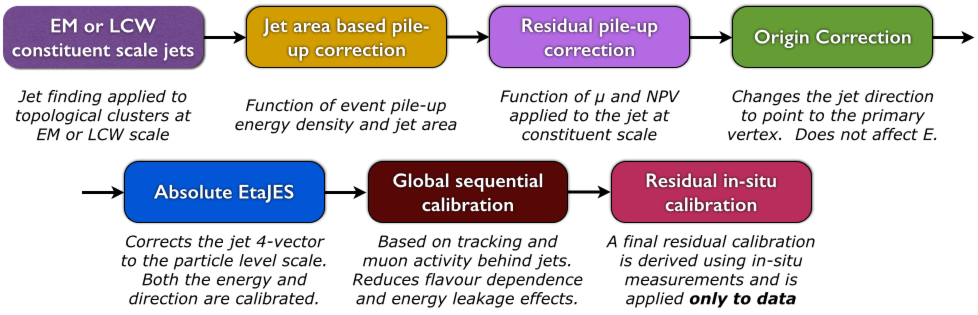
\includegraphics[width=1\textwidth]{chapters/c5/figures/jet_calib}
 \end{center}
 \caption{Calibration stages for reconstructed jets.}
 \label{fig:jet-calib}
\end{figure}
\par After jets are reconstructed, calibration needs to be applied on the four momentum of reconstructed jet to restore it back to particle-level energy scale.
A series of calibrations are applied after jet clustering as shown in Fig~\ref{fig:jet-calib}.

\begin{itemize}
\item \textbf{Origin correction} The kinematic observables of each topo-cluster are recalculated using the vector from the primary hard-scattering vertex to the topo-cluster centroid as its direction. The resolution of $\eta$ can be improved in this step. The jet energy is unaffected.
\item \textbf{Jet area-based pile-up correction} This step are designed to remove the excess energy from pile-ups. The area-based \pt density subtraction is applied event-by-event~\cite{Cacciari:2007fd}. The \pt density is estimated using the medium of \pt density of all jets in the event calculated by \pt/A, where A is the jet area.
\item  \textbf{Residual pile-up correction} A residual \pt  dependency on in-time pile-up $N_{PV}$ and out-of-time pile-up $\mu$ is roughly linear. So the linear correction is applied with coefficients derived from MC simulation.  
\item \textbf{Absolute MC-based calibration} An absolute jet energy and $\eta$ correction is derived from MC simulation. The average energy response is defined as the mean of $E_{reco}/E_{truth}$ binned in $E_{truth}$ and $\eta_{jet}$. Similar correction is done for $\eta$. 
\item \textbf{Residual in situ calibration} This steps aims at correcting difference between data and MC. For jets up to 950 GeV and with $|\eta|$< 0.8, Z+jest and $\eta$+jet balance is used, while, for high-pT jet  up to 2 TeV, multijet balance is used.
\end{itemize}

\begin{itemize}
\item \textbf{Trimming} This requires reclustering all of the jet’s constituents using the $k_T$ algorithm, which flavors clustering low \pt constituents first. This creates a set of subjets with radius parameter $R_{sub}$. Subjets with an energy below some threshold fraction of the energy of the large-R jet are removed from the large R jet. The trimmed large-R jet will be used to reconstruct Higgs candidates in boosted region.
\item \textbf{Pruning} Pruning is similar to trimming as it removes constituents with relative small $p_T$, while it has an additional wide-angle radiation veto. Large-R jets are first built with C/A or $anti-k_t$  algorithm. Constituents of ungroomed large-R jet are then re-clustered with C/A algorithm based on $R_{cut}$ and $Z_{cut}$. In each pairwise clustering step, secondary constituents with wide-angle $\Delta R_{12} > R_{cut} \times \frac{2M}/\pt$ or soft property are discarded. Definition of being soft is that $f_2 < Z_{cut}$ where $f_2$ is the fraction of softer constituent \pt with respect to the pair.

\end{itemize}


\subsection{Track jets}
\label{sec:track}
Sample text sample text sample text. Sample text sample text sample text.
Sample text sample text sample text. Sample text sample text sample text.
Sample text sample text sample text. Sample text sample text sample text.


\section{Missing Transverse Momentum (MET)}

\label{sec:met}
% What is MET
\par According to the conservation of momentum, the sum of the transverse memento of all particles produced in collisions is zero. Considering the existence of the non-detectable object, the transverse energies from detected objects are not balanced. The unbalanced part of transverse momentum is called ''missing transverse energy''(\met), or MET for short.

% How to calculate MET with/without Tracker fully involved.
\par As mentioned in the last paragraph, the \met~is derived by all other detectable objects. The \met~calculation is the most difficult object not only because it needs a full calculation of all detectable objects from various detectors, but also from the small fraction of energy deposits from unclustered parts of detectors. As a result, the \met~scale and \met~resolution are affected by many factors, such as missing Muons, mismeasured Jets, beam pile-up, etc. In the ATLAS experiment, the \met~reconstruction uses energy deposits in the calorimeters and muons tracks reconstructed in the muon detectors. Trackers' information is also used to recover the low Pt fraction that missed in the calorimeters \cite{ATLAS-CONF-2013-082}. Therefore, both hard objects (high \pt), like electrons, jets, muons, etc, and soft objects, like track soft terms, are considered in the \met~reconstruction.

% MET significance
\par The uncertainty of \met~calculation result can be remarkably large due to the complexity of the reconstruction algorithm. Therefore, a significance variable can be introduced to describe the reliability of the derived \met. The \met~significance is defined as
$$ S=\frac{\met}{\sqrt{\sum_{i}E_{Ti}}}, $$
where the numerator is the amplitude of derived \met, and the denominator is the scalar sum of the detected objects that used when to reconstruct the \met. A high value of \met~significance suggests the event is more likely to container invisible object rather than resolution smearing.
